\section{Propuesta de solución}

Reuniendo todo lo mencionado ante la problemática presente en la sociedad colombiana, que no se solucionará en el corto plazo, se propone una solución tecnológica \textit{temporal} que ayude a los pacientes a identificar un medicamento y encontrar alternativas cuando el fármaco original no esté disponible.

La solución planteada es implementar un sistema de IA que, a partir de una fotografía del medicamento (idealmente la \textbf{caja} o la \textbf{parte trasera del blíster}), permita: (i) reconocer el medicamento mediante extracción y verificación de texto (OCR) y (ii) recomendar alternativas farmacéuticas con base en el \textbf{principio activo principal}. El MVP se apoya en fuentes colombianas (INVIMA y \textit{Medicamentos a un Clic}) y en un motor de similitud basado en KNN.

\subsection{Prototipo de papel}

La Figura~\ref{fig:prototipo_papel} ilustra el prototipo conceptual del sistema, que define el flujo mínimo de interacción: captura/subida de imagen, verificación de texto detectado (OCR) y presentación de información y alternativas.

\begin{figure}[H]
	\centering
	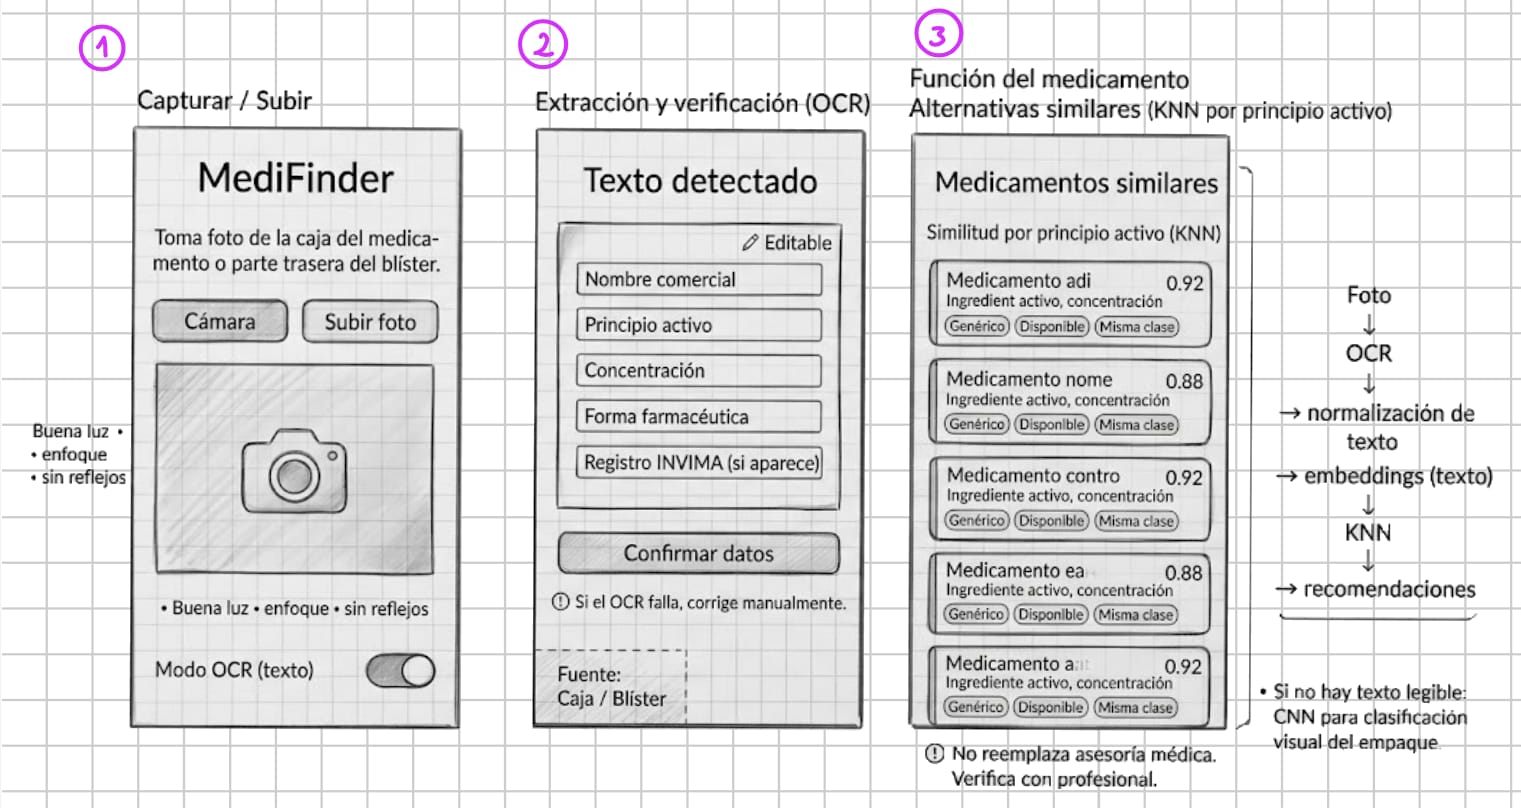
\includegraphics[width=0.97\textwidth]{img/prototipoPapel.png}
	\caption{Prototipo de papel (wireframe) del MVP de MediFinder: captura/subida, extracción y verificación (OCR) y resultados con función del medicamento y alternativas (KNN por principio activo).}
	\label{fig:prototipo_papel}
\end{figure}

\subsection{Prototipo de interfaz}

Además del wireframe en papel, se desarrolló un prototipo de interfaz digital para validar la experiencia de usuario y la navegación del MVP.

\begin{itemize}
	\item \textbf{Link de figma:} \href{https://city-wasp-51690509.figma.site/}{https://city-wasp-51690509.figma.site/}
	\item \textbf{Link Video demo:} \href{https://youtu.be/q5UDXb44g08}{https://youtu.be/q5UDXb44g08}
\end{itemize}

\begin{figure}[H]
	\centering
	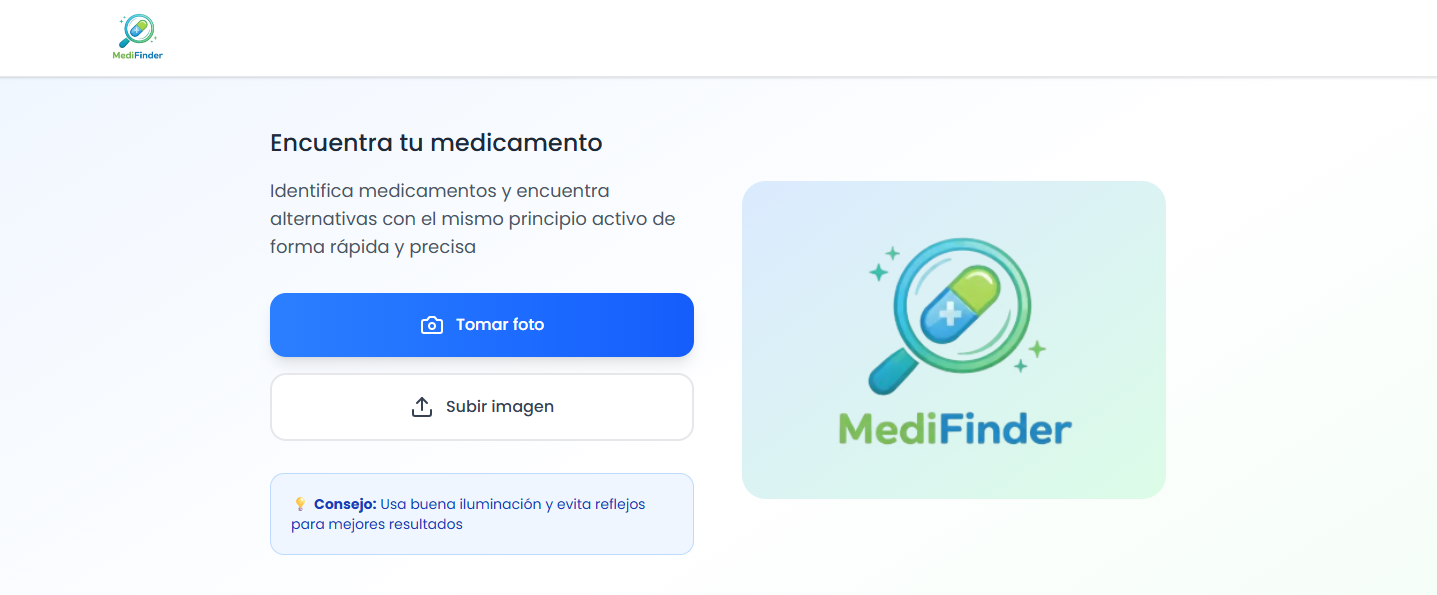
\includegraphics[width=0.9\textwidth]{img/prot1.png}
	\caption{Pantalla 1 del prototipo de interfaz de MediFinder.}
	\label{fig:prototipo_interfaz_1}
\end{figure}

\begin{figure}[H]
	\centering
	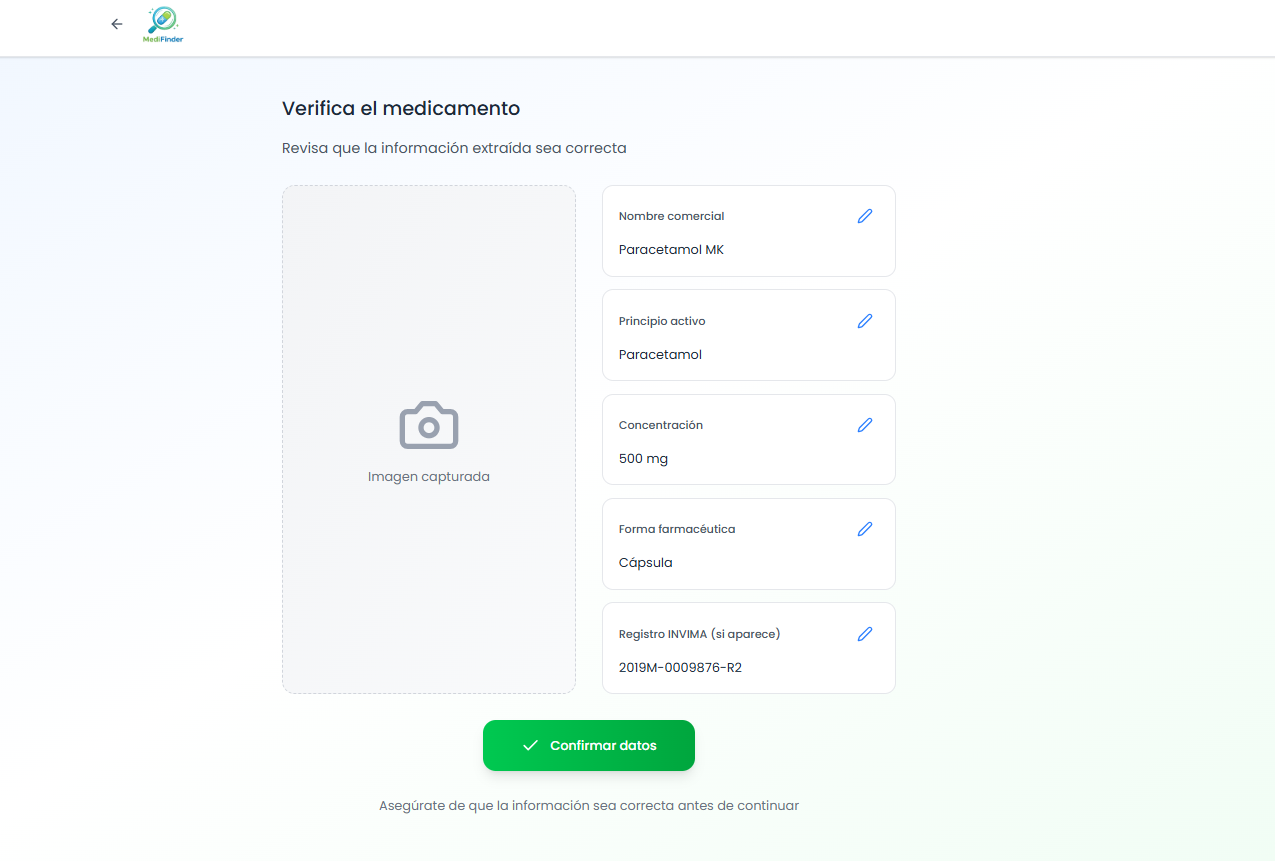
\includegraphics[width=0.9\textwidth]{img/prot2.png}
	\caption{Pantalla 2 del prototipo de interfaz de MediFinder.}
	\label{fig:prototipo_interfaz_2}
\end{figure}

\begin{figure}[H]
	\centering
	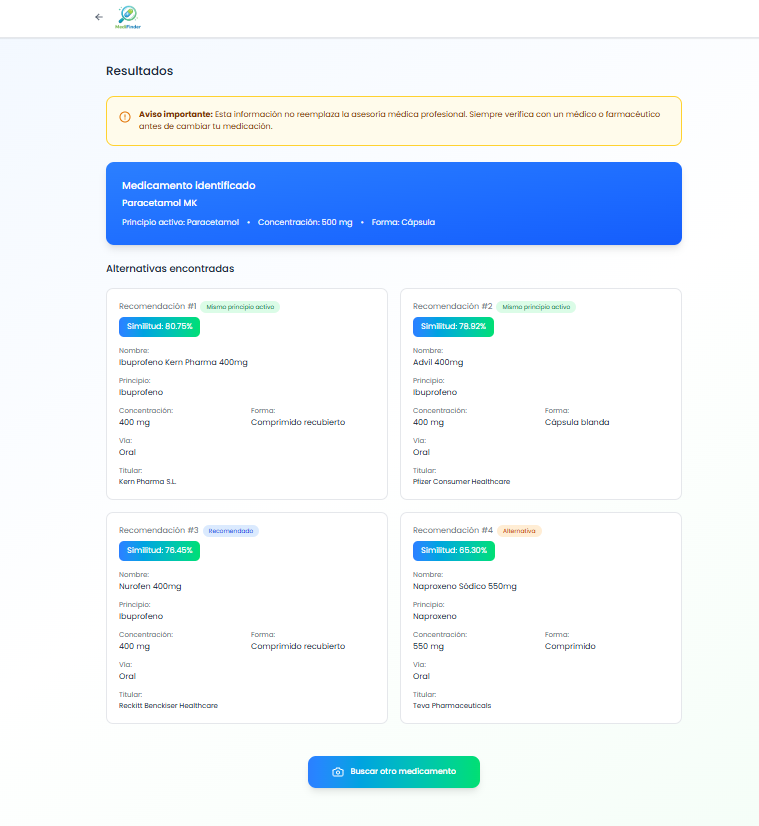
\includegraphics[width=0.9\textwidth]{img/prot3.png}
	\caption{Pantalla 3 del prototipo de interfaz de MediFinder.}
	\label{fig:prototipo_interfaz_3}
\end{figure}

\subsection{Arquitectura del sistema (MVP)}

El MVP se organiza como un pipeline en tres pasos, alineado con el flujo del prototipo:

\subsubsection{Paso 1: Captura de imagen y preprocesamiento}
\begin{itemize}
	\item El usuario toma o sube una imagen de la \textbf{caja del medicamento} o la \textbf{parte trasera del blíster}.
	\item Se aplica preprocesamiento para mejorar la legibilidad: corrección de rotación, ajuste de contraste y normalización del tamaño.
	\item Se muestran recomendaciones de captura (buena luz, enfoque y sin reflejos) para reducir errores.
\end{itemize}

\subsubsection{Paso 2: Extracción y verificación de texto (OCR + normalización)}
\begin{itemize}
	\item Se aplica OCR para extraer texto relevante del empaque/blíster (principalmente el \textbf{nombre del medicamento} y, cuando sea posible, concentración y forma farmacéutica).
	\item El sistema presenta los campos detectados de forma \textbf{editable} para que el usuario corrija errores frecuentes del OCR.
	\item Se normaliza el texto (tildes, mayúsculas/minúsculas, abreviaturas, unidades) y se realiza un proceso de \textit{matching} para mapear el texto a un registro del catálogo.
\end{itemize}

\subsubsection{Paso 3: Consulta de información y recomendación de alternativas (KNN)}
Una vez identificado el medicamento, el sistema:
\begin{itemize}
	\item consulta la información disponible en fuentes colombianas y el catálogo consolidado del proyecto;
	\item muestra la \textbf{función del medicamento} (tipo terapéutico y usos/indicaciones generales);
	\item calcula \textbf{alternativas similares} por \textbf{principio activo principal} usando KNN:
	\begin{itemize}
		\item \textbf{Prioridad 1 (equivalentes):} misma molécula (mismo principio activo principal) y, de ser posible, misma concentración y forma farmacéutica.
		\item \textbf{Prioridad 2 (similares por clase):} misma clase terapéutica cuando no existan suficientes equivalentes por molécula (se presenta como sugerencia informativa).
	\end{itemize}
\end{itemize}

\subsection{Fuentes de datos (Colombia) e integración}

El MVP se apoya en fuentes y plataformas con información relevante para Colombia:
\begin{itemize}
	\item \textbf{INVIMA} (listado de registros sanitarios de medicamentos) \cite{invima_registros}.
	\item \textbf{Medicamentos a un Clic} (consulta de información de medicamentos autorizados y regulados) \cite{medicamentosaunclic}.
\end{itemize}

En el prototipo, la información se consolida en un catálogo mínimo (por ejemplo CSV/JSON) para: (i) mapear el medicamento detectado a su principio activo principal y (ii) habilitar el ranking de alternativas por similitud.

\pagebreak